\documentclass[12pt]{article}
\usepackage[margin=1.0in]{geometry}
\usepackage{parskip}
\usepackage{graphicx}
\usepackage{minted}
\usepackage{xspace}

\setminted{autogobble,python3,mathescape,linenos,frame=lines,framesep=2mm,fontsize=\footnotesize}
\linespread{1.3}

\title{Project 9 --- Show and Tell}
% - The name of everyone in the group!
\author{
    Jonathan Sumner Evans (\texttt{jonathanevans@mines.edu})
    \and
    Sam Sartor (\texttt{ssartor@mines.edu})
    \and
    Daichi Jameson (\texttt{djameson@mines.edu})
}
\date{\today}

\newcommand{\app}{\textit{Show and Tell}\xspace}

\begin{document}
\maketitle

\section{Application Overview}
For our final project, we decided to build a web application for Mines students
to show off their cool projects on the ACM TV in Brown Building West. We call
the application \app after the age-old first-grade tradition. The core
functionality \app is that users can create teams and upload projects. These
projects are then verified by an system administrator, and once verified, the
projects are ready for display on the ACM TV.

% TODO: Sam, flesh this out

\subsection{Application Schema}
The core entities in our application are users, teams, and projects. In addition
to these entities, \app tracks user sessions and project assets. The following
ERD (Figure~\ref{fig:erd}) describes the relationships between these entities.

% TODO: Sumner, make nicer ERD diagram
\begin{figure}[H]
    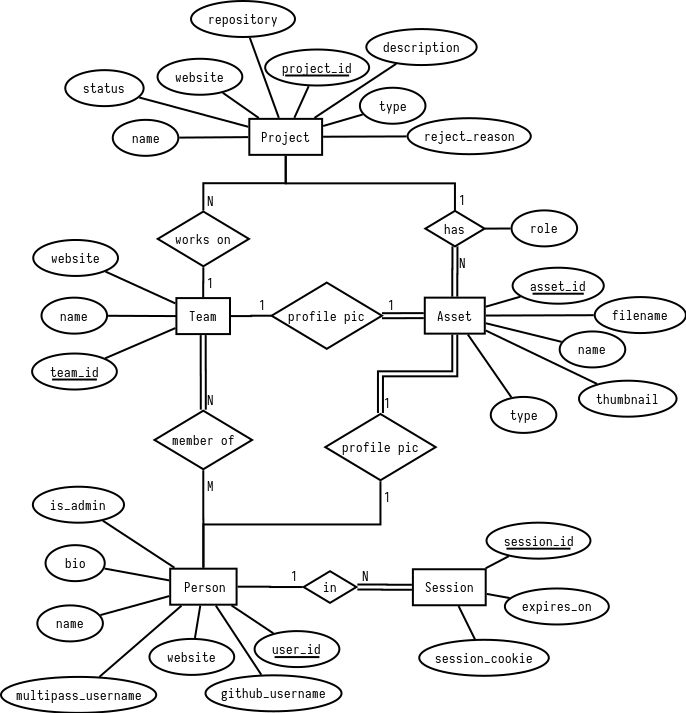
\includegraphics[width=\textwidth]{erd-new}
    \caption{The ERD for \app}
    \label{fig:erd}
\end{figure}

\subsection{Schema Explanation}
% TODO: Sumner

% - A section describing your dataset(s)
%
%     - What is interesting about this dataset?
%     - Where was the data obtained?
%     - What (if any) license restrictions are there on the use of the data?
%     - Describe the table or tables and significant attributes as loaded into the database.

\section{Application Implementation}
% - A section describing the awesome cool thing you did with your data. This
%   might include charts and data visualizations, screen captures of software,
%   interesting queries, and text descriptions.

% TODO: Sam, Daichi

\section{Implementation Difficulties}
% - A section describing the technical challenges you dealt with in obtaining,
%   manipulating, and loading the dataset(s).

% TODO: Each person contribute 1-2 things to this

\section{What We Learned}

% TODO: Each person contribute 1-2 things to this

\end{document}
